
\section{Linear Operators}

A common representation of NFAs is in terms of graphs,
which in turn are often represented by adjacency matrices,
adjacency lists, pointers, or some other representation.
Here we are concerned with adjacency matrices.
An interesting property of adjacency matrices is that they can be seen
as a function that maps between vertices on a graph.

This view is interesting for several reasons.
First, matrices are ways to represent linear operators
between finite-dimensional vector spaces.
Second, the space of linear operators can be endowed with a norm
known as the operator norm defined as follows:
\begin{align*}
  \norm{T}
    = \inf\braces{c \in \R \st
              \forall x \in X, \norm{Tx} \leq c \norm{x}_X}
\end{align*}
Where \(\type{T}{X}{Y}\) is a linear operator between
normed vector spaces \(X\) and \(Y\), which need not be finite-dimensional.
We remark that norm vector spaces that are complete with repsect to their
norm are called Banach spaces.
The definition of a norm like this allows us to then define a metric:
two operators are close in metric if their difference has a small norm.
The goal is to now extend this to the space of NFAs.
To do this, we first require a rigorous algebraic formulation of
formal language and automata theory, much of which is re-invented here.

There are several immediate problems to consider.
For one, it's not immediately obvious (if possible) how to embed
regular languages into an algebraic field,
which is required for a vector space.
Existing literature (much of what was also accidentally re-invented below)
on the algebraic study of formal language theory is grounded
in the language of (semi)-rings,
which has much weaker properties than what one may desire from a field.
Nevertheless, many properties from linear algebra can still be recovered,
although often with a caveat.
For instance, the lack of multiplicative inverses means that
matrix (linear operator) inverses are hard to compute,
or do not make much sense at first glance.
Because of this, we use the term linear space to do denote spaces
closed under linear operation, which may not have elements taken
over a field.

For a NFA \(A\), with \(A = \parens{\Sigma, Q, \Delta, S, F}\),
the goal is to view \(A\) acting as a linear operator between spaces.
In particular, the approach we take is to see \(\Delta\) as a
linear operator between spaces: this is perhaps the most obvious approach,
because to begin with, \(\Delta\) is already the transition function.

But the questions are then:
what are the appropriate linear spaces,
and what are the actions of the linear operator?
One initial thought is that the transition function can, in some way,
be seen as a directed acyclic graph on the states \(Q\),
where each edge is weighted by the letters in the alphabet \(\Sigma\)
that induce the transition.
The representation as an adjacency matrix does appear in
literature~\cite{savage1998models}.
Roughly, if \(M\) is the transition matrix, then \(M_{i, j} \in 2^{\Sigma}\)
denotes the states that will transition state \(q_i\) to \(q_j\).

While such a matrix representation is useful,
it is not immediately obvious how such a matrix does indeed correspond
to a linear operator, especially on what linear spaces.
One possible interpretation is to see
the linear spaces as \(\abs{Q}\)-dimensional,
where each dimension of the space corresponds to one member of \(Q\).
The objects of the space is then sets of strings over \(\Sigma\).

\begin{definition}[String Space]
  The string space of \(\Sigma\) is a semiring
  \(\parens{2^{\Sigma^\star}, \cup, \cdot, \zero, \one}\)
  such that:
  \begin{enumerate}
    \item[(a)]
      The semiring addition is the set union
      \(\type{\cup}{2^{\Sigma^\star} \times
        2^{\Sigma^\star}}{2^{\Sigma^\star}}\).

    \item[(b)]
      The semiring multiplication is the string concatenation
      \(\type{\cdot}{2^{\Sigma^\star} \times
        2^{\Sigma^\star}}{2^{\Sigma^\star}}\)
      such that:
      \begin{align*}
        A \cdot B
          = \braces{a \cdot b \st a \in A, b \in B}
      \end{align*}
  \end{enumerate}
\end{definition}

Here the string space is the power set of all strings generated
by \(\Sigma\) through monoid multiplication (string concatenation).
Defining the string space like this allows us to equip it with a semiring
structure by viewing addition as set union.
For convenience,
we may write \(R\) instead of \(2^{\Sigma^\star}\)
to denote the set corresponding to the string space.

Observe that \(R\) has the structure of a \(1\)-dimensional linear space.
The big difference, however, is that the scalar elements are
elements of a semiring rather than a field.
Nevertheless, \(R\) is still closed under linear operations,
and is therefore a linear space.

\begin{theorem}
  A string space \(R\) is a linear space.
\end{theorem}
\begin{proof}
  A semiring contains a zero element and is closed under
  (semiring) addition.
  Furthermore,
  it is closed under (left semiring) multiplication
  with respect to other elements of the semiring.
\end{proof}

The natural extension of a \(1\)-dimensional linear space
is a \(n\)-dimensional linear space.

\begin{definition}[\(n\)-String Space]
  For a string space \(R\) and \(n \in \Zp\),
  the \(n\)-dimensional string space \(R^n\) is then the
  free semimodule isomorphic to \(n\) copies of \(R\).
\end{definition}

A natural representation of \(R^n\) is as a \(n\)-dimensional vector,
and in this case we prefer row vectors to column vectors.
We abuse notation to identify elements of \(R^n\) with their
row vector representation.
Furthermore, we demonstrate that this is indeed still a linear space,
where semiring operations are defined coordinate-wise.
An immediate consequence is that this also forms a linear space,
since it is an \(n\)-dimensional linear space.


In particular, it would be nice to have a linear operator
between string spaces.

\begin{definition}[Linear String Space Operator]
  A linear string space operator
  is a linear operator \(\type{A}{R^n}{R^m}\).
\end{definition}

In particular, we are interested in a matrix representation.

\begin{definition}[Matrix Representation of Linear String Space Operator]
  The matrix representation of a linear string space operator
  \(\type{A}{R^n}{R^m}\) is a matrix
  \(A \in M_{n \times m} \parens{R}\) that
  acts on row vectors of \(R^n\) by right multiplication.
\end{definition}

Here each entry of the matrix denotes the sets strings that are
concatenated during transition.
As with the \(n\)-dimensional string space \(R^n\),
we abuse notation for \(A\) to stand in for
both the linear operator and its matrix representation.
From linear algebra, we know that the space of linear operators between
linear spaces is itself a linear space.

Observe that the elements for the matrix of \(A\) are drawn from
\(R\) (which is just \(2^{\Sigma^\star}\))
rather than \(2^{\Sigma}\),
which is what we would expect for an NFA.
In other words, transitions in \(A\) are given by sets of potentially
long strings, rather than just single alphabets.
The definition provided here is intended to be slightly more general,
with the NFA case of single-letter transitions being a special case.
Nevertheless,
given a NFA, we are now ready to describe a particular matrix representation
as a linear operator between \(n\)-string spaces.

\begin{definition}[Matrix Representation of \(\Delta\)]
  For a NFA \(\parens{\Sigma, Q, \Delta, S, F}\) with
  string space \(R\) generated by \(\Sigma\) and \(n = \abs{Q}\),
  the matrix representation of \(\Delta\) as a linear operator
  is a matrix
  \(A \in M_{n \times n} \parens{R}\)  where:
  \begin{align*}
    A_{i, j}
      = \braces{a \st \parens{\parens{a, q_i}, B} \in \Delta, q_j \in B}
  \end{align*}
\end{definition}

Of course, this is a linear string space operator simply because
every entry of the transition matrix will be a set of singleton strings.




\begin{example}
  Consider \(\Sigma = \braces{a, b, c}\) and the NFA below:

  \begin{figure}[h!]
  \centering
  \begin{tikzpicture}
    [->,
     >=stealth',
     shorten >=1pt,
     auto,
     node distance=2cm,
     semithick,
     state/.style={circle, draw, minimum size=1cm} 
    ]
    \node[state] (Q1) at (0, 0) {\(q_1\)};
    \node[state] (Q2) at (3, 1.5) {\(q_2\)};
    \node[state] (Q3) at (3, -1.5) {\(q_3\)};

    \path (Q1) edge [] node
              {\(\braces{a, b}\)} (Q2);
    \path (Q2) edge [loop right] node
              {\(\braces{a}\)} (Q2);
    \path (Q2) edge [] node
              {\(\braces{b}\)} (Q3);
    \path (Q3) edge [loop right] node
              {\(\braces{a, c}\)} (Q3);
    \path (Q3) edge [] node
              {\(\braces{c}\)} (Q1);
  \end{tikzpicture}
  \caption{NFA Graph}
  \end{figure}
  The most important distinction between this and a typical
  NFA is that we implicitly assume every state to be both starting
  and accepting.
  In other words, accepting strings is very permissive,
  which simplifies things for now.
  However,
  to embed this into our model there are several steps.

  First, we have the string space
  \(\parens{2^{\Sigma^\star}, \bigcup, \cdot, \zero, \one}\).

  Next, for the matrix \(A\) that we will construct,
  take \(A_{i, j}\) to denote the transition from state
  \(q_i\) to state \(q_j\).
  The matrix is then:
  \begin{align*}
    A =
      \begin{bmatrix}
        \zero & \braces{a, b} & \zero \\
        \zero & \braces{a} & \braces{b} \\
        \braces{c} & \zero & \braces{a, c}
      \end{bmatrix}
  \end{align*}
  In order to perform string concatenation towards the right,
  transition matrices act by right-matrix multiplication.
  That is, if \(v \in R^3\) is the initial \(n\)-dimensional
  string space, then the subsequent string space is \(v A\).

  To briefly demonstrate, two transitions of the matrix \(A\) appears as
  follows:
  \begin{align*}
    A^2 =
      \begin{bmatrix}
        \zero & \braces{a, b} & \zero \\
        \zero & \braces{a} & \braces{b} \\
        \braces{c} & \zero & \braces{a, c}
      \end{bmatrix} 
      \begin{bmatrix}
        \zero & \braces{a, b} & \zero \\
        \zero & \braces{a} & \braces{b} \\
        \braces{c} & \zero & \braces{a, c}
      \end{bmatrix}
      =
      \begin{bmatrix}
        \zero & \braces{aa, ba} & \braces{ab, bb} \\
        \braces{bc} & \braces{aa} & \braces{ab, ba, bc} \\
        \braces{ac, cc} & \braces{ca, cb} & \braces{aa, ac, ca, cc}
      \end{bmatrix}
  \end{align*}
  In general, from graph theory, \(A^k\) denotes the \(k\)th consecutive
  transition using \(A\),
  and each entry \(A^k _{i, j}\) is the set of strings that will
  get from state \(q_i\) to \(q_j\) in \(k\) steps.

\end{example}


\subsection{Automata Metrics}

Having established how to embed (regular) languages into linear spaces
with NFAs as linear operators between these spaces,
we now turn our attention to defining a metric over NFAs.


\subsubsection{Edit Distance Metrics}
Matrices are a common representation of linear operators between
finite-dimensional linear spaces.
Our first attempt is based on graph edit distance,
which directly corresponds with matrix edit distance.
We that in retrospect this was not a good idea,
and experimental results were bad.
Nevertheless, we proceed.

Our main objective here is to define a syntactic metric
based on graph edit distance in addition to a semantic metric
derived from earlier work with measure theory.
First, we quickly recap the measure-based metrics.

\begin{definition}[String Space Measure]
  Let
  \(\parens{\Sigma^\star, \sigma\parens{\Sigma^\star}}\)
  be a measurable space defined on the strings \(\Sigma^\star\).
  If \(\type{\lambda}{\sigma\parens{\Sigma^\star}}{\Rz}\) is a measure,
  then we call it a string space measure,
  and the measure space
  \(\parens{\Sigma^\star, \sigma\parens{\Sigma^\star}, \lambda}\)
  a string measure space.
\end{definition}

The elements of a string measure space consists of strings finite,
while the \(\sigma\)-algebra generated consists of sets of finite strings.
A measure \(\type{\lambda}{\sigma\parens{\Sigma^\star}}{\Rz}\) is also
equipped, and may be defined.
We have also shown previously that
measures are able to define a metric.

\begin{definition}[String Space Metric]
  Let
  \(\parens{\Sigma^\star, \sigma\parens{\Sigma^\star}, \lambda}\)
  be a string measure space.
  The string metric space \(\parens{\powset{\Sigma^\star}, \zeta}\) is
  a metric space with a metric function
  \(\type{\zeta}{\powset{\Sigma^\star} \times \powset{\Sigma^\star}}{\Rz}\)
  defined as:
  \begin{align*}
    \zeta \parens{A, B}
      = \lambda\parens{A \triangle B}
  \end{align*}
\end{definition}
\begin{theorem}
  The string space metric function
  \(\type{\zeta}{\powset{\Sigma^\star} \times \powset{\Sigma^\star}}{\Rz}\)
  is a metric function.
\end{theorem}
\begin{proof}
  The function induced by a measure and the symmetric set difference
  is a metric.
\end{proof}

Recall that although we write \(\powset{\Sigma^\star}\) here,
they are synonymous with \(R\).
Having defined a metric on string spaces,
we are interested in examining how we may
syntactically compare two linear operators
between string spaces.
To do this, we formalize the notion of edit distance on matrices
in terms of algebra.

First, for two operators
\(\type{A_1, A_2}{R^n}{R^m}\), it is possible that
the two are isomorphic up to some permutation.
Note that we want to consider the special case of \(n = m\) first,
for which theories of permutation matrix related to
graph isomorphism are well-developed.
After all, we are focused on NFAs here,
which have nice an straightforward graph (matrix) representations.

\begin{theorem}[Square Operator Permutation]
  Let \(P_n \subseteq M_{n \times n}\parens{R}\)
  denote the family of \(n\)-dimensional permutation matrices.
  Two linear operators
  \(\type{A_1, A_2}{R^n}{R^n}\) are isomorphic if
  there is a permutation matrix
  \(P \in P_n\) such that:
  \begin{align*}
    A_1 = P A_2 {P}^T
  \end{align*}
\end{theorem}
\begin{proof}
  The action of permutation matrices on the matrix representation on
  a graph is equivalent to relabelling the vertices,
  which preserves graph (and thus operator) isomorphism.
\end{proof}

Permutation matrices give us the ability to talk about
isomorphisms up to permutation.
However they lack the ability to talk about how
syntactically similar two matrices might be up to permutation.
To do this, for two matrices of the same dimensions,
we may be interested in seeing how far the image of the matrices
in each dimension differ.
Without permutation matrices
for two matrices \(A\) and \(B\), we may try something like this:
\begin{align*}
  \sup_{1 \leq i, j \leq n}
    \zeta\parens{A_{i, j}, B_{i, j}}
\end{align*}
In other words, we find entries of the matrix that yield the most distance
with respect to the \(\zeta\) string space metric function.
With permutation matrices, we may try something like this:
\begin{align*}
  \inf_{P \in P_n} \sup_{1 \leq i, j \leq n}
    \zeta\parens{A_{i, j}, B_{i, j}}
\end{align*}
This is fairly straightforward, and more or less just amounts to saying
to take the best permutation of one of the matrices with respect
to the other, and then take the distance with respect to
\(\zeta\).

However, there are still several concerns here.
First, we need to generalize this to cases where
\(A\) and \(B\) are not the same dimension.
In addition, we are not completely sure if taking the infimum of
\(P \in P_n\) retains a metric structure,
which means that such an operation may need to be defined with respect
to a fixed permutation matrix.

We first consider how square matrices of different dimensions may be compared.

\begin{definition}[Linear Operator Dimension]
  Let \(\type{A}{R^n}{R^n}\) be a square linear string space operator.
  For \(m > n\),
  the dimension extension of \(A\)
  is a square linear operator \(\type{\overline{A}}{R^m}{R^m}\)
  whose matrix representation has form:
  \begin{align*}
    \overline{A} = \begin{bmatrix} A & \zero \\ \zero & \zero \end{bmatrix}
  \end{align*}
\end{definition}

Although the newly appended dimensions of operator action
effectively have trivial action, this still acts as an embedding into
a higher dimension.
With this, we then attempt to define a metric between
two square linear matrices of different dimensions:
\begin{definition}[Non-Uniform Dimension Square Linear Operator Metric]
  For two square linear operators
  \(\type{A}{R^n}{R^n}\) and \(\type{B}{R^m}{R^m}\) where \(m > n\),
  fix the permutation matrix \(P \in P_m\),
  define the operator metric
  \(\type{Z_{p, n, m}}
      {\parens{R^n \to R^n} \times \parens{R^m \to R^m}}{\Rz}\) as:
  \begin{align*}
    Z_{p, n, m}\parens{A, B} =
      \sup_{1 \leq i, j \leq m}
        \zeta\parens{\overline{A}_{i, j}, \parens{PB{P}^T}_{i, j}}
  \end{align*}
\end{definition}
In short, when given two square linear matrices
\(A\) and \(B\) where \(A\)
is a smaller dimension than \(B\), the goal of the metric function \(Z\)
is to first stretch \(A\) into \(\overline{A}\)
to match the dimension of \(B\),
and then apply the supremum coordinate-wise metric
on \(\overline{A}\) and \(B\).

\begin{theorem}
  The function
  \(\type{Z_{p, n, m}}
      {\parens{R^n \to R^n} \times \parens{R^m \to R^m}}{\Rz}\) 
  defined above is a metric.
\end{theorem}
\begin{proof}
  Once the permutation matrix \(P \in P_m\) is fixed, this reduces to
  applying the supremum over a finite set of metric functions
  for each entry of the matrix.
\end{proof}

The challenge, of course, is finding the correct permutation matrix \(P\).
We note that although we used the supremum here, another viable option
could be general \(p\)-norm type summations,
which also do induce a metric because they satisfy the triangle inequality.

Nevertheless, the painstaking process here allows us to
algebraically formalize
an edit distance metric for matrix representations of NFA.


\begin{example}
  Consider \(\Sigma = \braces{a, b, c}\) and two NFAs defined below:

  \begin{figure}[h!]
  \centering
  \begin{minipage}{0.45\textwidth}
  \begin{tikzpicture}
    [->,
     >=stealth',
     shorten >=1pt,
     auto,
     node distance=2cm,
     semithick,
     state/.style={circle, draw, minimum size=1cm} 
    ]
    \node[state] (Q1) at (0, 0) {\(q_1\)};
    \node[state] (Q2) at (3, 1.5) {\(q_2\)};
    \node[state] (Q3) at (3, -1.5) {\(q_3\)};

    \path (Q1) edge [] node
              {\(\braces{a}\)} (Q2);
    \path (Q2) edge [loop above] node
              {\(\braces{b}\)} (Q2);
    \path (Q2) edge [] node
              {\(\braces{a}\)} (Q3);
    \path (Q3) edge [] node
              {\(\braces{c}\)} (Q1);
  \end{tikzpicture}
  \caption{NFA \(A\)}
  \end{minipage}%
  \begin{minipage}{0.45\textwidth}
  \begin{tikzpicture}
    [->,
     >=stealth',
     shorten >=1pt,
     auto,
     node distance=2cm,
     semithick,
     state/.style={circle, draw, minimum size=1cm} 
    ]
    \node[state] (Q1) at (0, 0) {\(q_2\)};
    \node[state] (Q2) at (3, 1.5) {\(q_3\)};
    \node[state] (Q3) at (3, -1.5) {\(q_4\)};
    \node[state] (Q4) at (6, 0) {\(q_1\)};
  

    \path (Q1) edge [] node
              {\(\braces{a}\)} (Q2);
    \path (Q2) edge [loop above] node
              {\(\braces{b}\)} (Q2);
    \path (Q2) edge [] node
              {\(\braces{a}\)} (Q3);
    \path (Q3) edge [] node
              {\(\braces{c}\)} (Q1);
    \path (Q2) edge [] node
              {\(\braces{c}\)} (Q4);
    \path (Q4) edge [] node
              {\(\braces{a}\)} (Q3);

  \end{tikzpicture}
  \caption{NFA \(B\)}
  \end{minipage}
  \end{figure}
  The respective transition matrices are then:
  \begin{align*}
    A =
      \begin{bmatrix}
        \zero & \braces{a} & \zero \\
        \zero & \braces{b} & \braces{a} \\
        \braces{c} & \zero & \zero
      \end{bmatrix}
    \qquad
    \overline{A} =
      \begin{bmatrix}
        \zero & \braces{a} & \zero & \zero \\
        \zero & \braces{b} & \braces{a} & \zero \\
        \braces{c} & \zero & \zero & \zero \\
        \zero & \zero & \zero & \zero
      \end{bmatrix}
    \qquad
    B =
      \begin{bmatrix}
        \zero & \zero & \zero & \braces{a} \\
        \zero & \zero & \braces{a} & \zero \\
        \braces{c} & \zero & \braces{b} & \braces{a} \\
        \zero & \braces{c} & \zero & \zero
      \end{bmatrix}
  \end{align*}

  The corresponding permutation matrix is:
  \begin{align*}
    P =
      \begin{bmatrix}
        \zero & \one & \zero & \zero \\
        \zero & \zero & \one & \zero \\
        \zero & \zero & \zero & \one \\
        \one & \zero & \zero & \zero
      \end{bmatrix}
  \end{align*}
  Indeed, we have:
  \begin{align*}
    PB{P}^T
    =
      \begin{bmatrix}
        \zero & \one & \zero & \zero \\
        \zero & \zero & \one & \zero \\
        \zero & \zero & \zero & \one \\
        \one & \zero & \zero & \zero
      \end{bmatrix}
      \begin{bmatrix}
        \zero & \zero & \zero & \braces{a} \\
        \zero & \zero & \braces{a} & \zero \\
        \braces{c} & \zero & \braces{b} & \braces{a} \\
        \zero & \braces{c} & \zero & \zero
      \end{bmatrix}
      \begin{bmatrix}
        \zero & \zero & \zero & \one \\
        \one & \zero & \zero & \zero \\
        \zero & \one & \zero & \zero \\
        \zero & \zero & \one & \zero
      \end{bmatrix}
    =
      \begin{bmatrix}
        \zero & \braces{a} & \zero & \zero \\
        \zero & \braces{b} & \braces{a} & \braces{c} \\
        \braces{c} & \zero & \zero & \zero \\
        \zero & \zero & \braces{a} & \zero
      \end{bmatrix}
  \end{align*}
  If we proceed with the metric \(\zeta\) calculation
  (assuming a counting measure) at each entry.
  We find the most significant differences occur
  at row-column index pairs \(\parens{2, 4}\) and \(\parens{4, 3}\):
  \begin{align*}
    \zeta_{\parens{2, 4}}\parens{\overline{A}_{2, 4},
           \parens{PB{P^T}}_{2, 4}}
      = \zeta_{\parens{2, 4}}\parens{\zero, \braces{c}} = 1
    \qquad
    \zeta_{\parens{4, 3}} \parens{\overline{A}_{4, 3},
           \parens{PB{P^T}}_{4, 3}}
      = \zeta_{\parens{4, 3}}\parens{\zero, \braces{a}} = 1
  \end{align*}

\end{example}

The experiments here did not work.
In simulations run,
there was very poor correlation between the syntactic graph edit distance
metric with the semantic measure-based metric.

In part this may be because a small edit in a graph may induce a large
change in the language accepted.
For instance, disconnecting a single edge
means that up to (countably) infinitely many words are no longer
recognized by the automata that the graph represents.

This suggests that other syntactic metrics may be necessary,
but nevertheless this is a preliminary step towards
our goal.


\subsubsection{Bi-Directional Merging}


\begin{minipage}{0.45\textwidth}
\begin{center}
  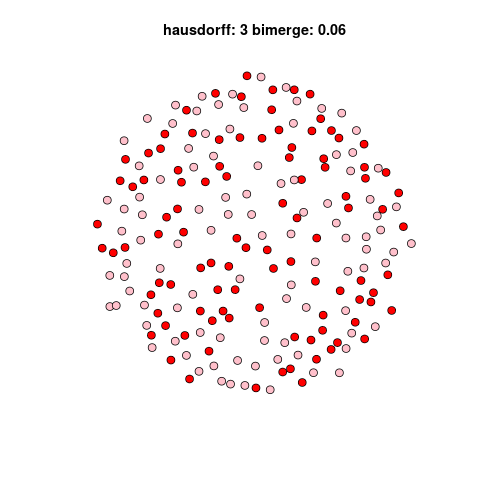
\includegraphics[scale=0.5]{images/AD6-AD6-100-IM.png}
\end{center}
\end{minipage}
\begin{minipage}{0.45\textwidth}
\begin{center}
  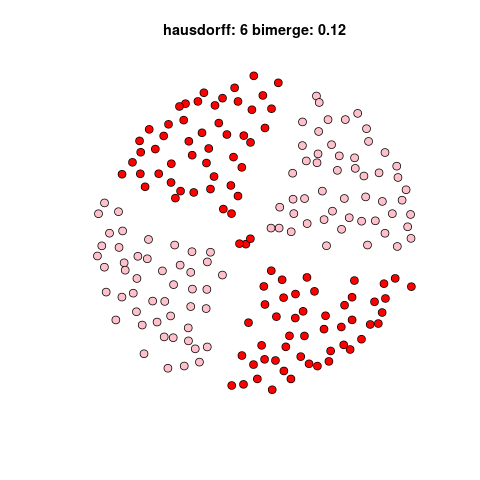
\includegraphics[scale=0.5]{images/AD6-DG6-100-IM.png}
\end{center}
\end{minipage}





